\section{Controllability Analysis}

A full controllability analysis was performed on the system to establish whether:

\begin{enumerate}
	\item The system has adequate set point tracking characteristics.
	\item The system has adequate disturbance rejection characteristics.
\end{enumerate}

The method used is described in [REF!!]. 

\subsection{Minimal Realisation of the System}

The system written in the transfer function notation is in no danger of not being a minimal realizable system. It is only when the system is converted to state space notation it runs the risk of not being a minimal realization. 

When converting the transfer function model to a state space realisation of the system, it has to be noted that all dead time that is inherent to the system is ignored, as state space realizations cannot deal with dead time. The system was however converted to its state space realization, in order to cross check the calculated poles and zeros of the system.

The minimum state space realization of the system is given below.

\subsection{Functional Controllability}

The system has to be checked for functional controllability. This implies that outputs should be able to be controlled independently. There are two factors that have to be considered when checking for functional controllability of a system, namely

\begin{enumerate}
	\item There have to be at least as many inputs as there are outputs
	\item The rank of G(s) should be greater than the number of outputs.
\end{enumerate} 

For consideration 1, mentioned above, the number of inputs and outputs in the system is equal. This criteria is therefore satisfied by the system.

For consideration 2, the minimum singular value (or $\underline{\sigma}$) of $G(j\omega)$ should be non-zero. In order to determine whether the system satisfies this criteria, all the singular values, of all the outputs were computed of a wide frequency range. A bode diagram displaying the result can be seem in Figure~\ref{fig:gs-singular-values}.

\begin{figure}
	\centering
	\includegraphics[width=0.7\linewidth]{"Figures/G(s) Singular Values"}
	\caption{The singular values of $G(j\omega)$.}
	\label{fig:gs-singular-values}
\end{figure}

As is clear from Figure~\ref{fig:gs-singular-values}, $\underline{\omega}$ never reaches zero, although it does approach zero as the frequency goes to infinity. 

Based on the above information, is can be concluded that the system is indeed functional controllable. This means that the system's rank is equal to the amount of outputs that the system has.

The current selected inputs and outputs can therefore be controlled with adequate independence.

\subsection{System Poles}

\subsubsection{Calculating the System Poles}

The poles of the system was calculated. The system has a total  number of six poles. The poles calculated are described in the Table~\ref{tab: Poles of system}.

\begin{table}[H]
	\centering
	\caption{The poles of the system.}
	\begin{tabular}{ccc}
		\hline
		\textbf{Pole} & \textbf{Real Part} & \textbf{Imaginary Part} \\\hline
		$p_1$            & -0.3923            & 0                       \\
		$p_2$            & -0.1397            & 0                       \\
		$p_3$            & -0.0791            & 0.0349                  \\
		$p_4$            & -0.0791            & -0.0349                 \\
		$p_5$            & -0.0960             & 0.0042                  \\
		$p_6$            & -0.0960             & -0.0042   \\\hline             
	\end{tabular}
	\label{tab: Poles of system}
\end{table}

\subsubsection{Calculating the System Pole Directions}

The pole directions of the system was calculated by substituting all the pole values into $G(s)$ and calculating the input and output directions of the relevant poles. The calculated pole direction are given Table~\ref{tab: Pole Directions of system}.

\begin{table}[H]
	\centering
	\caption{The pole directions of the system.}
	\begin{tabular}{ccc}
		\hline
		\textbf{Pole} & \textbf{Input Direction ($V$)} & \textbf{Output Direction ($U$)} \\\hline
		$p_1$            &$ \begin{bmatrix} 0.34 \\ 0.94 \\ -0.04\end{bmatrix} $ & $ \begin{bmatrix} 0.80 \\ -0.07 \\ 0.60\end{bmatrix} $ \\
		$p_2$            & $ \begin{bmatrix} -0.15 \\ 0.19 \\ 0.97\end{bmatrix} $ & $ \begin{bmatrix} -0.05 \\ -0.05 \\ 1.00\end{bmatrix}$ \\
		$p_3$            & $ \begin{bmatrix} -0.59 \\ -0.12 - 0.13j \\ -0.76 - 0.02j\end{bmatrix} $ & $ \begin{bmatrix} -0.11 -0.07j \\ 0.03 - 0.03j \\ -0.78 - 0.61j\end{bmatrix} $\\
		$p_4$            & $ \begin{bmatrix} -0.59 \\ -0.12 + 0.13j \\ -0.76 + 0.02j\end{bmatrix} $ & $ \begin{bmatrix} -0.11 +0.07j \\ 0.03 + 0.03j \\ -0.78 + 0.61j\end{bmatrix} $\\
		$p_5$            & $ \begin{bmatrix} -0.71 \\ 0.14 -0.19j \\ -0.66 +0.04j\end{bmatrix} $ & $ \begin{bmatrix} -0.31+0.56j \\ 0.31+0.55j \\ -0.09 -0.43j\end{bmatrix} $ \\
		$p_6$            & $ \begin{bmatrix} -0.71 \\ 0.14 +0.19j \\ -0.66 -0.04j\end{bmatrix} $ & $ \begin{bmatrix} -0.31-0.56j \\ 0.31-0.55j \\ -0.09 +0.43j\end{bmatrix} $ \\\hline             
	\end{tabular}
	\label{tab: Pole Directions of system}
\end{table}

\subsubsection{Discussion of System Poles}

\subsection{System Zeros}

\subsubsection{Calculating the System Zeros}

The system zeros were calculated. The system contains a total number of nine zeros, all of them located in the left hand plane (LHP). The system zeros are given in Table~\ref{tab: Zeros of system}.

\begin{table}[H]
	\centering
	\caption{The zeros of the system.}
	\begin{tabular}{ccc}
		\hline
		\textbf{Zero} & \textbf{Real Part} & \textbf{Imaginary Part} \\\hline
		$z_1$            & -0.3077            & 0                       \\
		$z_2$            & -0.2571            & 0                       \\
		$z_3$            & -0.2            & 0                  \\
		$z_4$            & -0.1493            & 0                 \\
		$z_5$            & -0.1227             & 0                  \\
		$z_6$            & -0.1157             & 0   \\
		$z_7$            & -0.1104             & 0   \\
		$z_8$            & -0.0917             & 0   \\
		$z_9$            & -0.0532             & 0   \\\hline             
	\end{tabular}
	\label{tab: Zeros of system}
\end{table}

\subsubsection{Calculating the System Zero Directions}

The zero directions of the system was calculated by substituting all the zero values into $G(s)$ and calculating the input and output directions of the relevant zeros using the singular value decomposition of $G(z_i)$. The calculated zero directions are given Table~\ref{tab: Zero Directions of system}.

\begin{table}[H]
	\centering
	\caption{The zero directions of the system.}
	\begin{tabular}{ccc}
		\hline
		\textbf{Zero} & \textbf{Input Direction ($V$)} & \textbf{Output Direction ($U$)} \\\hline
		$z_1$            &$ \begin{bmatrix} 1 \\ 0 \\ 0\end{bmatrix} $ & $ \begin{bmatrix} 0 \\ 1 \\ 0\end{bmatrix} $ \\
		$z_2$            &$ \begin{bmatrix} 0 \\ 0 \\ 1\end{bmatrix} $ & $ \begin{bmatrix} 0 \\ 0 \\ 1\end{bmatrix} $ \\
		$z_3$            &$ \begin{bmatrix} 0 \\ -1 \\ 0\end{bmatrix} $ & $ \begin{bmatrix} 0 \\ 1 \\ 0\end{bmatrix} $ \\
		$z_4$            &$ \begin{bmatrix} -1 \\ 0 \\ 0\end{bmatrix} $ & $ \begin{bmatrix} -1 \\ 0 \\ 0\end{bmatrix} $ \\
		$z_5$            &$ \begin{bmatrix} -1 \\ 0 \\ 0\end{bmatrix} $ & $ \begin{bmatrix} 0 \\ 0 \\ 1\end{bmatrix} $ \\
		$z_6$            &$ \begin{bmatrix} 0 \\ 1 \\ 0\end{bmatrix} $ & $ \begin{bmatrix} -1 \\ 0 \\ 0\end{bmatrix} $ \\
		$z_7$            &$ \begin{bmatrix} 0 \\ 0 \\ 1\end{bmatrix} $ & $ \begin{bmatrix} -0.707 \\ -0.707 \\ 0\end{bmatrix} $ \\
		$z_8$            &$ \begin{bmatrix} 0 \\ 1 \\ 0\end{bmatrix} $ & $ \begin{bmatrix} 0 \\ 0 \\ 1\end{bmatrix} $ \\
		$z_9$            &$ \begin{bmatrix} 0 \\ 0 \\ 1\end{bmatrix} $ & $ \begin{bmatrix} 0 \\ 0 \\ 1\end{bmatrix} $ \\\hline             
	\end{tabular}
	\label{tab: Zero Directions of system}
\end{table}

\subsubsection{Discussion of System Zeros}


\begin{figure}[H]
	\centering
	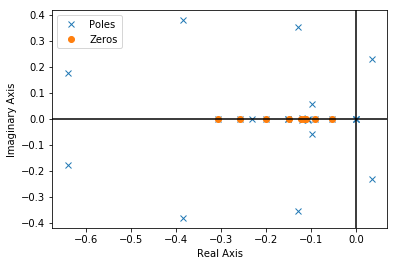
\includegraphics[width=0.7\linewidth]{Figures/Poles_and_Zeros}
	\caption{A graphical representation of the system's poles and zeros.}
	\label{fig:polesandzeros}
\end{figure}

